\section{实验与分析}\label{sec:2.3}
\subsection{数据收集与预处理}\label{subsection:2.3.1}
为测试在线负面口碑处理专家识别的准确性,本文从中关村在线进行数据采集。
该平台是中国专业的IT与数码门户网站,
用户可在该平台发布抱怨问题、提出解决方案、搜索和浏览其他用户沉淀的历史内容。
平台会根据用户的活跃程度计算等级,并根据用户参与问答的情况赋予用户专家称号,
这些专家用户均经过平台审核,可信度较高,是进行专家识别实验的理想数据。

数据收集过程如下:
从中关村在线网站分类栏目中“手机”领域的所有11940位用户作为数据源进行数据爬取。
爬取内容主要包括用户手机领域回答历史、提问与回答数量、累计回答等级、累计推荐等级和平台个人等级。
因本文主要研究在线负面口碑处理的专家识别,重点关注专家用户,故在此删除提问数量数据,
并去除其中未发表或标记提问与回答数据的用户10771位,保留关注用户1169位。
其中,因网页格式差异等原因导致部分用户数据爬取不完整,删除28位数据缺失用户后,保留有效用户1141位。

数据预处理过程如下:
由于本文模型与算法均在文本数据的前提下进行设计,
因此实验将用户回答历史中图片、视觉符号等非文本数据剔除。
回答文本中同时存在较多的散列标签,它们作为句子的一部分存在,而又仅作为引用标签,
故本文从历史回答文本中通过正则表达式去除了无意义的散列标签。
为实现多样化的表达,用户可以使用重复符号和表情符号来表达特定情绪,
由于本文基于情感词典分析用户情感,这些符号并未被词典收录,故在此去除重复符号和表情符号。
此外,为保护用户隐私,实验通过哈希变换对用户ID进行了加密处理。

在完成了必要的数据收集和预处理后,本文从11940位用户中获取到1169位关注用户,
其中28位用户缺失部分数据,
故最终保留1141位有效用户数据作为实验样本数据。部分用户数据示例如表3所示。
\begin{table}[ht]
    \centering
    \caption{用户数据示例}\label{tab:2.3}
    \vskip -10pt
    \begin{tabularx}{\textwidth}{YccYcY}
    \toprule
    用户ID & 知识文档相似度 & 平均情感得分 & 回答数 & 累计推荐等级 & 等级\\
    \midrule
    29637408 & 0.03863 & 3.49927 & 12 & 1 & 1 \\
    29792448 & 0.26281 & 7.40783 & 1529 & 3 & 34  \\
    29452432 & 0.02664 & 4.71405 & 157 & 1 & 23  \\
    29797317 & 0.44034 & 5.96295 & 719 & 4 & 12  \\
    29797439 & 0.44079 & 6.29400 & 1247 & 3 & 25  \\
    \bottomrule
    \end{tabularx}
\end{table}

为避免量纲不同对模型的影响,对所有指标数据进行归一化处理,具体为:
\begin{equation}\label{eq:2.4}
    f_i=\frac{f^{'}_i - f_{\min}}{f_{\max}-f_{\min}}
\end{equation}

其中$f_i$表示指标的测量值$f^{'}_i$归一化后的对应值,
$f_{\min}$表示所有样本在此指标测量真实值中的最小值,
$f_{\max}$表示所有样本在此指标测量真实值中的最大值。

实验从归一化后的1141个样本用户数据中随机抽取80\%共913位用户作为训练集对支持向量机进行训练,
训练通过松弛变量和惩罚参数调整分类超平面,以实现分类收敛。
将剩下的20\%共228位用户作为测试集,评估模型效果。

\subsection{实验设计与分析}\label{subsection:2.3.2}
实验将在线负面口碑处理的专家识别问题转化为分类问题,并选用SKlearn-SVM包完成分类任务。
在专家识别实验之前,先构建用于分析用户回答记录文档的词库,并基于该词库进行知识水平的计算。
为提高对用户文档分词的准确率,利用现有词库(包括手机词汇大全、通讯与数码产品词汇等),
加入网络流行语、口语方言等词语,构成新的分词词库,
基于该词库对用户文档进行分词,计算用户的领域知识水平;
利用扩充后的情感词典计算用户情感状态;利用爬取的数据计算用户互动程度。

在专家识别实验中,以领域知识水平、情感状态和互动程度这三类特征的7种不同组合
$C_{DKL \& SS \& SD}$、$C_{DKL}$、$C_{SS}$、$C_{SD}$、$C_{DKL \& SS}$、$C_{DKL \& SD}$)和$C_{SS \& SD}$
建立支持向量机分类模型实现专家识别,通过结果分析选取效果最好的组合。

关于评价指标,实验采用标准机器学习分类评价指标(准确率、精确率、召回率和$F_1$值)
对专家识别效果进行评价。
根据上述实验设计和评价指标设定,在线负面口碑专家识别的结果如\autoref{tab:2.4}、\autoref{fig:2.1}所示。
\begin{table}[ht]
    \centering
    \caption{专家识别实验结果}\label{tab:2.4}
    \vskip -10pt
    \begin{tabularx}{\textwidth}{lYcccccc}
    \toprule
    模型 & $C_{DKL \& SS \& SD}$ & $C_{DKL}$ & $C_{SS}$ & $C_{SD}$ & $C_{DKL \& SS}$ & $C_{DKL \& SD}$ & $C_{SS \& SD}$ \\
    \midrule
    准确率 & 0.8805 & 0.7622 & 0.8054 & 0.8125 & 0.8595 & 0.8135 & 0.8270  \\
    精确率 & 0.8892 & 0.9533 & 0.9380 & 0.9062 & 0.8935 & 0.9677 & 0.9007  \\
    召回率 & 0.9557 & 0.5514 & 0.6541 & 0.7632 & 0.8162 & 0.6486 & 0.7351  \\
    $F_1$ & 0.9213 & 0.6987 & 0.7707 & 0.8286 & 0.8531 & 0.7767 & 0.8095  \\
    \bottomrule
    \end{tabularx}
\end{table}

\begin{figure}[th]
    
    \centering
    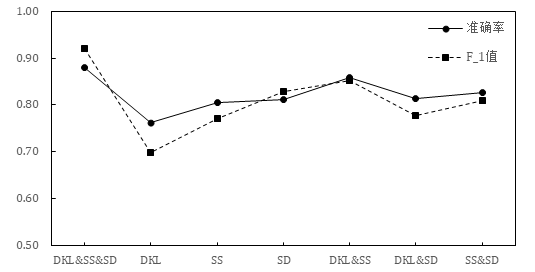
\includegraphics[width=0.9\textwidth]{figure2-1.png}
    \vskip -10pt
    \caption{模型准确率与$F_1$值折线图}\label{fig:2.1}
\end{figure}

由\autoref{tab:2.4}和\autoref{fig:2.1}可知,
在线负面口碑处理的专家识别实验中综合考虑用户知识水平、情感状态和互动程度的分类模型
$C_{DKL \& SS \& SD}$效果最佳
(其中准确率为88.05\%,精确率为88.92\%,召回率为95.57\%和$F_1$值为92.13\%,
准确率和$F_1$值皆明显大于其他模型),
这说明模型$C_{DKL \& SS \& SD}$在专家识别中具有明显优势。
在单类特征模型中,$C_{SD}$和$C_{SS}$ 的效果均优于$C_{DKL}$,
其中$C_{SD}$与$C_{SS}$的差别并不显著,这说明专家用户相对普通用户拥有更正面的情感状态和更高的互动程度。
在两类特征模型中,$C_{DKL \& SS}$的效果较优,$C_{SS \& SD}$次之,$C_{DKL \& SD}$较劣,
但三者与$C_{DKL}$和$C_{SS}$之间差距亦不显著,且皆优于$C_{DKL}$,
这说明本文定义的情感状态和互动程度相较领域知识水平更有助于在线负面口碑处理的专家识别,
尽管领域知识水平也可用于专家识别,但其显著性低于综合特征分类模型和其他特征分类模型。

综上所述,本文实验有如下发现:
(1)情感状态和互动程度相比领域知识水平更有助于进行在线负面口碑处理的专家识别;
(2)单独的领域知识水平特征不能很好的进行在线负面口碑处理的专家识别,
考虑领域知识水平、情感状态和互动程度三者混合的特征分类模型可以显著提高专家识别的准确率和总体效果。